\documentclass[article]{abntex2}
\usepackage[alf]{abntex2cite}
\usepackage{graphicx} 
\usepackage[utf8]{inputenc}
\usepackage{url}
\usepackage[portuguese]{babel}

\title{IF728- ENGENHARIA DE SISTEMAS EMBUTIDOS}
\author{Mateus Alves Nunes da Rocha}
\date{16 de Setembro de 2022}

\begin{document}

\maketitle
\section{Introdução}

\paragraph{}
O sistema embutido é um sistema de hardware e softwareprojetado para executar tarefas específicas em um sistemamaior. Eles são integrados a outros produtos ouequipamentos para controlar ou monitorar funções ouprocessos específicos. Esses sistemas geralmente sãoprojetados para serem simples e baratos, consistindo emcomponentes limitados (como microcontroladores, sensores eatuadores). \cite{embarcados}

No \textbf{Centro de Informática (CIn) da UFPE}, adisciplina de Infra-estrutura de Hardware é pré-requisitopara IF728, que aprofunda nos conceitos de metodologia,implementação e ferramentas de apoio ao desenvolvimento desistemas embutidos.
    
\section{Relevância}

\paragraph{}
Inúmeros outros equipamentos fazem uso de sistemasembarcados, como: impressoras, calculadoras, máquinas delavar, cafeteiras eletrônicas, semáforos, fotossensores,aparelhos de TV e termômetros digitais.
    
Os sistemas embarcados já fazem parte da vida das pessoas,dando destaque ao meio IoT (Internet of Things) e ao meioindustrial. A Internet das Coisas está relacionada àinclusão de sensores e software em vários dispositivospara que eles possam se comunicar e enviar dados pelaInternet. \cite{inove}
    

\subsection{Aplicações de Sistemas Embutidos}
\begin{itemize}
    \item MP3 Player
    
        \paragraph {}
        Além de ser capaz de armazenar músicas em sua memória interna, o dispositivo ainda realizava outras funções, como tocar as faixas registradas, sintonizar estações de rádio e gravar áudio.Embora atualmente ultrapassado pelos smartphones, é um ótimo exemplo de embarcado que fez parte da vida das pessoas.
        
    \item Roteador
    
        \paragraph {}
        O roteador pode ser descrito como um dispositivo desenvolvido com a finalidade de conectar aparelhos, como computadores e smartphones, a uma rede, como o wi-fi.

 \end{itemize}
 
\begin{figure}[h]
\caption{Roteador}
\label{figura:abba1}
\centering
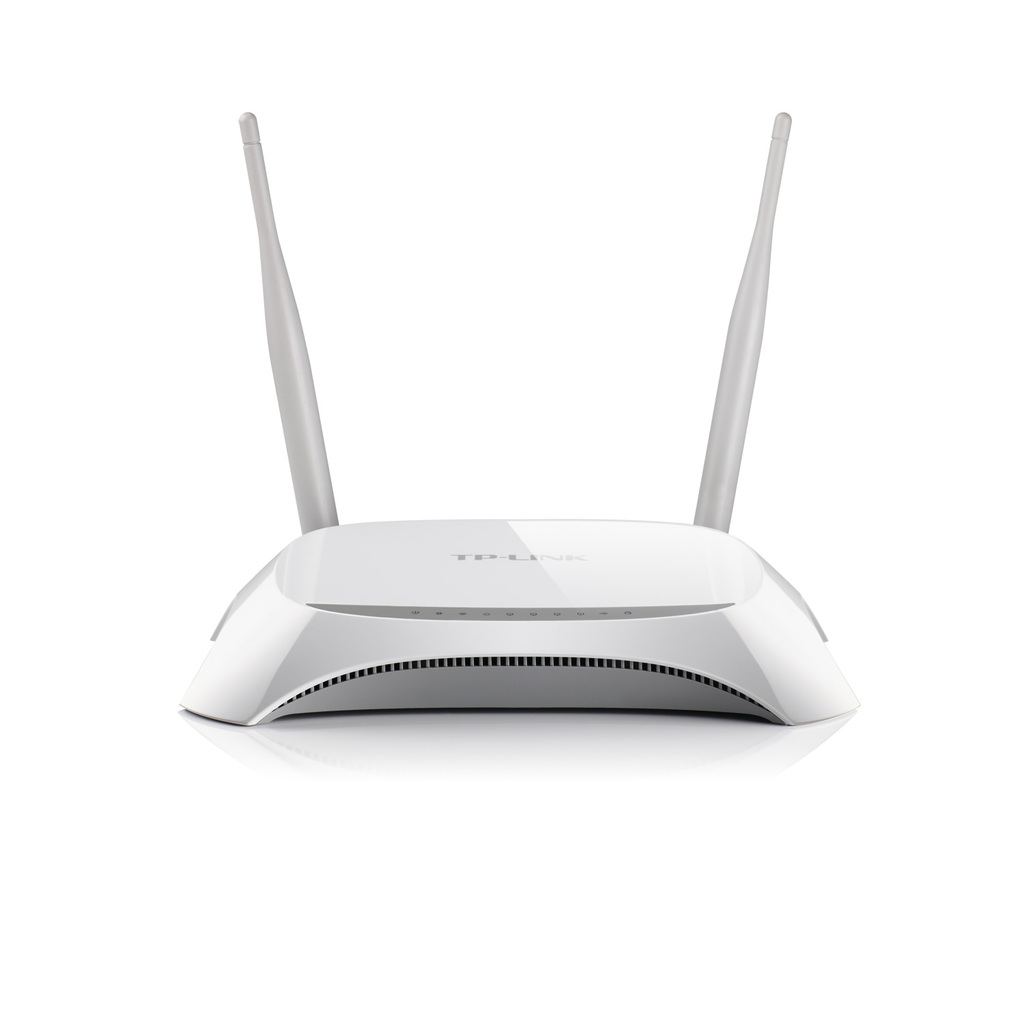
\includegraphics[width=5cm]{master_roteador-wireless-tp-link-300n-3g-4g-2-antenas-tl-mr3420-1507399d.jpg}
\end{figure}


\begin{figure}[h]
\caption{MP3 player}
\label{figura:abba2}
\centering
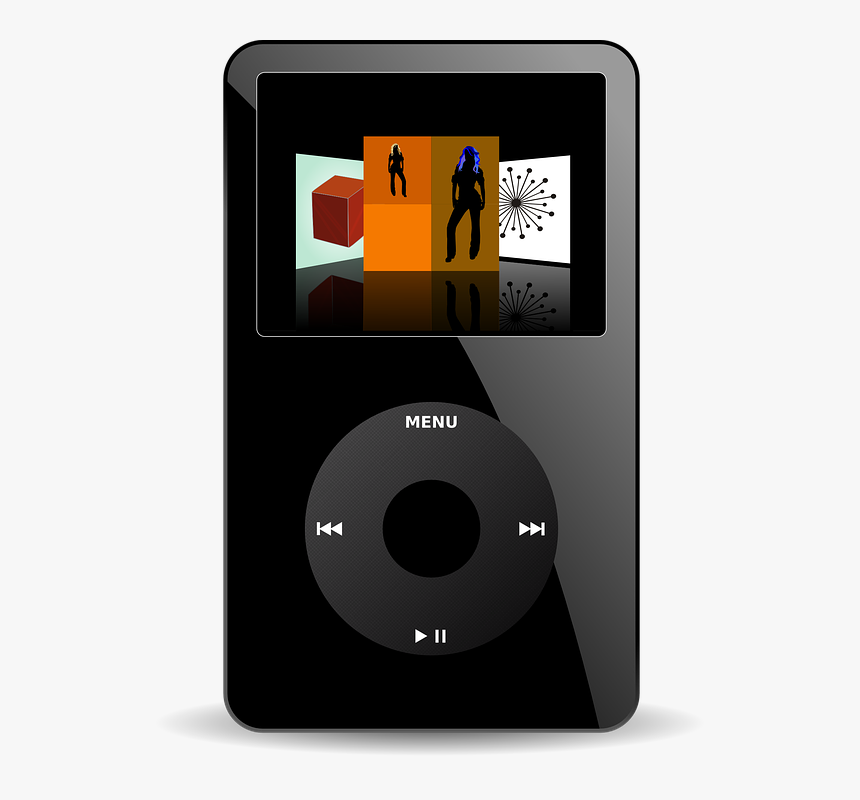
\includegraphics[width=5cm]{504-5040308_mp3-player-png-transparent-png.png}
\end{figure}

\section{Relação com outras disciplinas}

\paragraph{}
A cadeira de Engenharia de Sistemas Embutidos tem várias braches no mercado, desde roteadores a sistemas de gerenciamento de táxis \cite{sistemaTaxis}

Por isso, pode ser linkada com várias outras cadeiras oferecidas pelo CIn. Entre essas cadeiras, podemos citar: IF674- INFRA-ESTRUTURA DE HARDWARE (Bom entendimento do equipamento a ser utilizado); IF729 - PROTOTIP. DE CIRCUITOS INTEGRADOS (Essencial devido à necessidade da composição de placas para os projetos de S.E.) e IF730 - SISTEMA DE TEMPO REAL (Essencial para garantir a robustez do sistema e a eficiência do mesmo)


\bibliography{references}

\end{document}
